% ------------------------------------------------------------------------------
% TYPO3 CMS 7.4 - What's New (English Version)
%
% @author	Michael Schams <schams.net>
% @license	Creative Commons BY-NC-SA 3.0
% @link		http://typo3.org/download/release-notes/whats-new/
% @language	English
% ------------------------------------------------------------------------------
% LTXE-CHAPTER-UID:		0dbe76ce-5948c314-454b95fd-543cb62c
% LTXE-CHAPTER-NAME:	Interfaz de Usuario de Backend
% ------------------------------------------------------------------------------

\section{Interfaz de Usuario de Backend}
\begin{frame}[fragile]
	\frametitle{Interfaz de Usuario de Backend}

	\begin{center}\huge{Capítulo 1:}\end{center}
	\begin{center}\huge{\color{typo3darkgrey}\textbf{Interfaz de Usuario de Backend}}\end{center}

\end{frame}

% ------------------------------------------------------------------------------
% LTXE-SLIDE-START
% LTXE-SLIDE-UID:		464d4ba6-dab07499-0cd5f168-552e9729
% LTXE-SLIDE-ORIGIN:	8080f469-3c5592f0-dc25ad87-894c2648 German
% LTXE-SLIDE-TITLE:		Feature: #48947 - Avatars for backend users
% LTXE-SLIDE-REFERENCE:	Feature-48947-AvatarsForBackendUsers.rst
% ------------------------------------------------------------------------------
\begin{frame}[fragile]
	\frametitle{Interfaz de Usuario de Backend}
	\framesubtitle{Avatares para Usuarios de Backend}

	Para mejorar la experiencia de usuario en la edición colaborativa de contenido, ahora los usuarios del backend pueden usar avatares.
	Estas pequeñas imágenes de usuario se muestran en la barra superior, en la lista de usuarios y otros lugares.

	\begin{figure}
		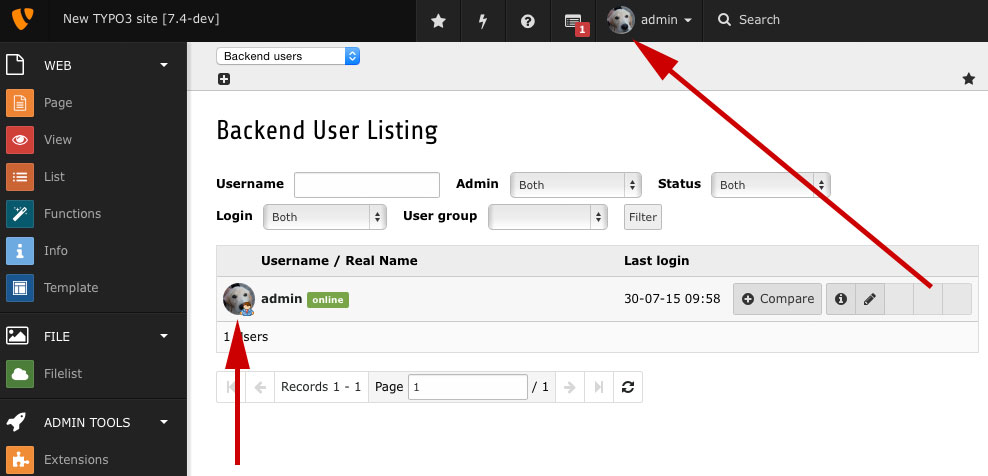
\includegraphics[width=0.65\linewidth]{BackendUserInterface/48947.jpg}
	\end{figure}

\end{frame}

% ------------------------------------------------------------------------------
% LTXE-SLIDE-START
% LTXE-SLIDE-UID:		89f348c8-db045eff-5dfc4f42-da1a2cfa
% LTXE-SLIDE-ORIGIN:	b0f7e15a-7cc72aaa-79738ec7-643c5cec German
% LTXE-SLIDE-TITLE:		Feature: #56133 - Replace file feature for fal file list
% LTXE-SLIDE-REFERENCE:	Feature-56133-ReplaceFileFeatureForFalFileList.rst
% ------------------------------------------------------------------------------
\begin{frame}[fragile]
	\frametitle{Interfaz de Usuario de Backend}
	\framesubtitle{Reemplazar Ficheros}

	Los ficheros en la lista de registros FAL pueden ahora ser \textbf{reemplazados} (requiere "vista extendida" habilitada).
	El nombre de fichero del archivo existente puede ser mantenido o actualizado.

	\begin{figure}
		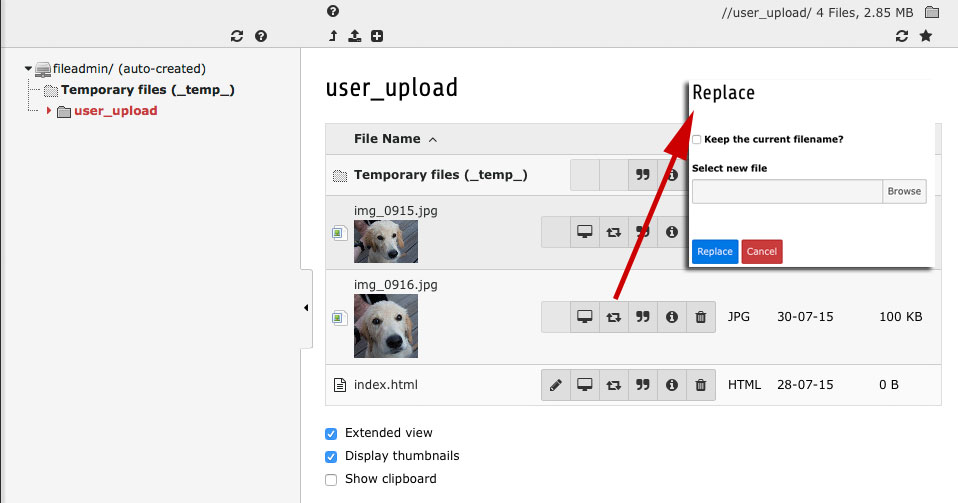
\includegraphics[width=0.75\linewidth]{BackendUserInterface/56133.jpg}
	\end{figure}

\end{frame}

% ------------------------------------------------------------------------------
% LTXE-SLIDE-START
% LTXE-SLIDE-UID:		7e5987f7-9a91ea61-8564c721-0f8d5e4a
% LTXE-SLIDE-ORIGIN:	613354cc-9475feef-bec620c5-31170549 German
% LTXE-SLIDE-TITLE:		Feature: #67574 - Display online status in backend user list
% LTXE-SLIDE-REFERENCE:	Feature-67574-DisplayOnlineStatusInBackendUserList.rst
% ------------------------------------------------------------------------------
\begin{frame}[fragile]
	\frametitle{Interfaz de Usuario de Backend}
	\framesubtitle{Estado en línea de los Usuarios del Backend}

	El estado online de los usuarios del backend se muestra en el módulo "Usuarios de Backend".

	\begin{figure}
		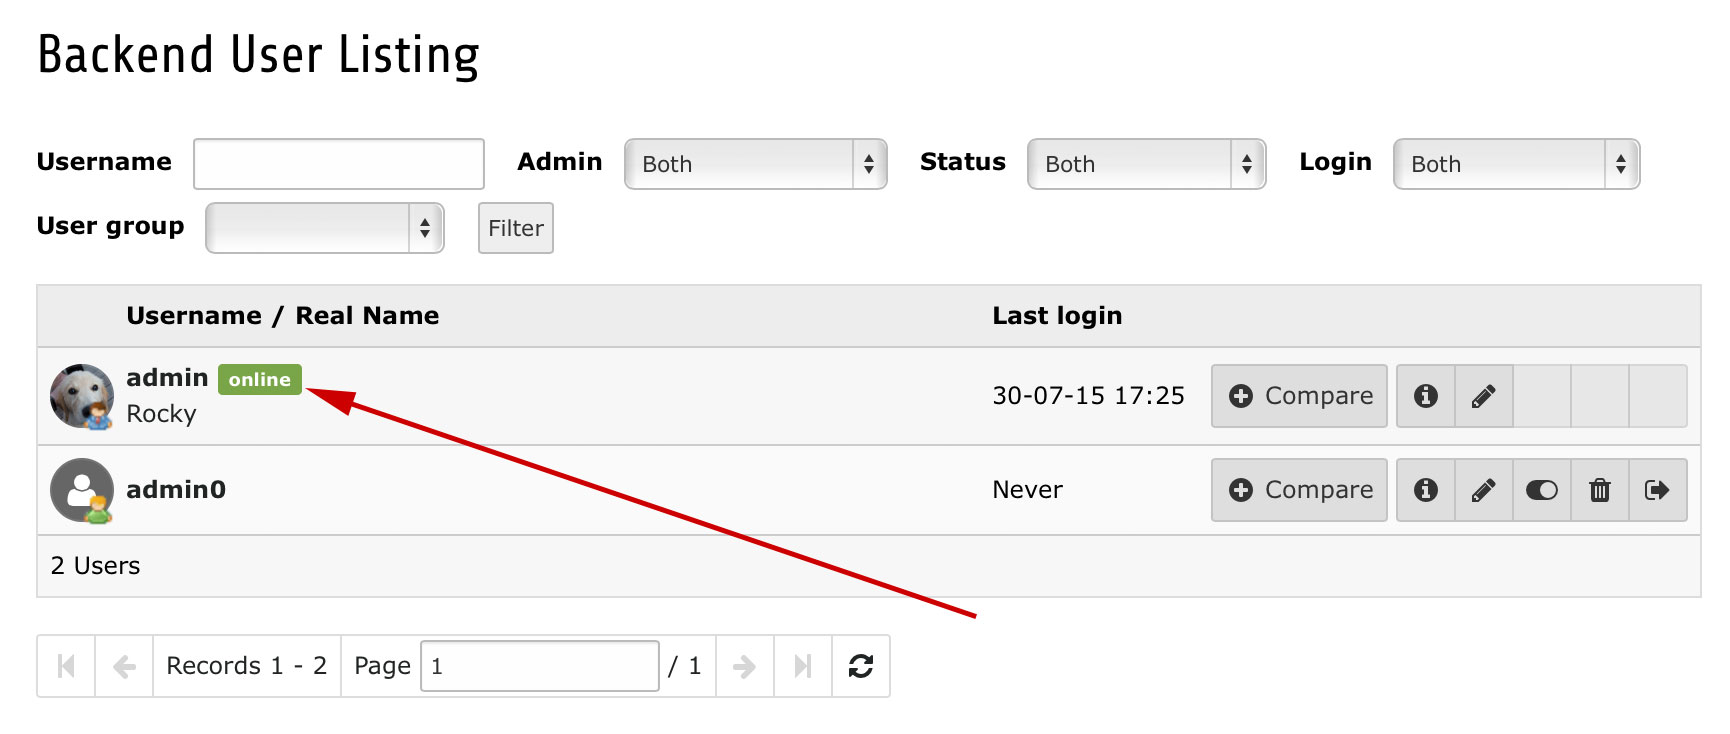
\includegraphics[width=0.9\linewidth]{BackendUserInterface/67574.jpg}
	\end{figure}

\end{frame}

% ------------------------------------------------------------------------------
% LTXE-SLIDE-START
% LTXE-SLIDE-UID:		0154fc51-74683590-ebbe8559-ce6a0d57
% LTXE-SLIDE-ORIGIN:	00c93fe2-9d128591-20b71814-13556f43 German
% LTXE-SLIDE-TITLE:		FormEngine: Drop "Show secondary options"
% LTXE-SLIDE-REFERENCE:	https://forge.typo3.org/issues/67753
% ------------------------------------------------------------------------------
\begin{frame}[fragile]
	\frametitle{Interfaz de Usuario de Backend}
	\framesubtitle{Eliminadas Opciones Secundarias}

	Se han eliminado el checkbox "Mostrar opciones secundarias (paletas)", la opción de TSconfig de página \texttt{options.enableShowPalettes}
	y la configuración de TCA. Las paletas están siempre visibles y no pueden esconderse más.

	\begin{figure}
		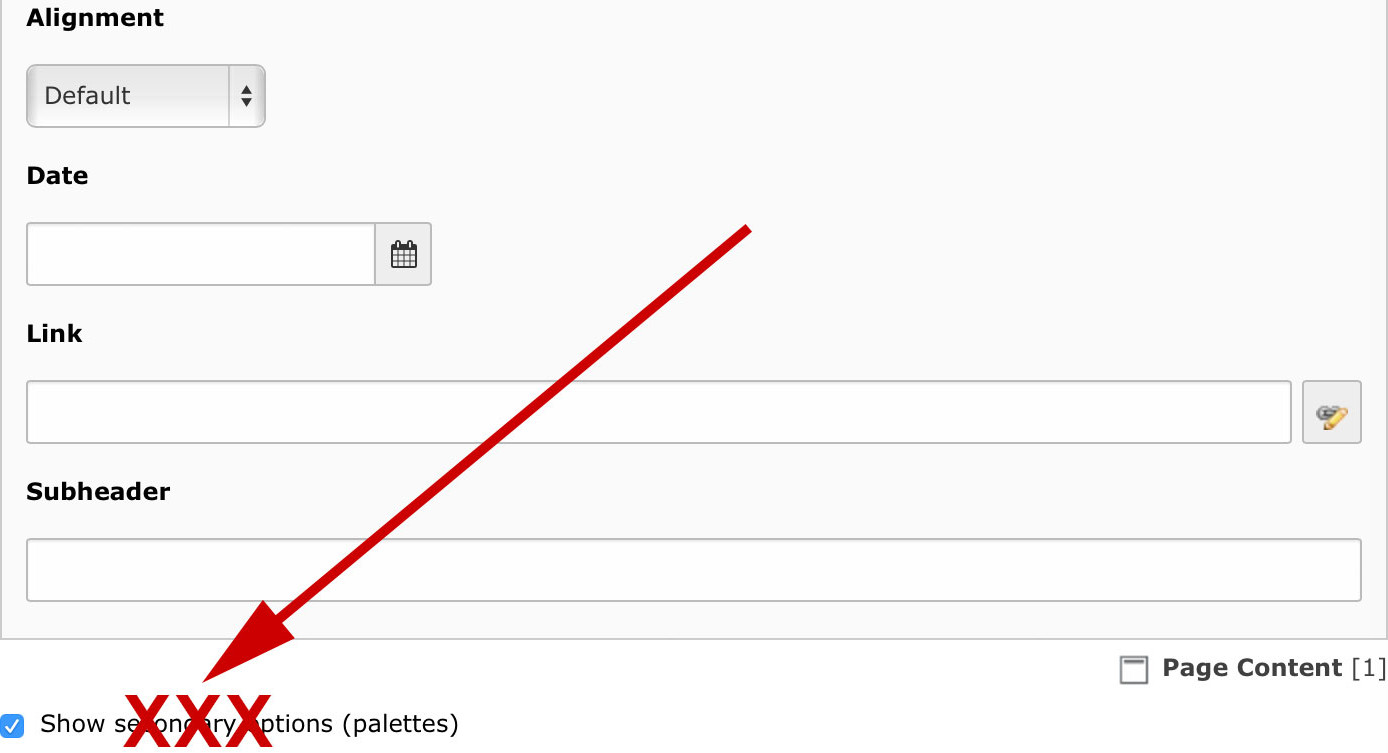
\includegraphics[width=0.6\linewidth]{BackendUserInterface/67753.jpg}
	\end{figure}

\end{frame}

% ------------------------------------------------------------------------------
% LTXE-SLIDE-START
% LTXE-SLIDE-UID:		f9b24e36-28e8872c-41297de9-52467554
% LTXE-SLIDE-ORIGIN:	bab4e93d-0a6d4612-41b2f67e-47c37ff7 German
% LTXE-SLIDE-TITLE:		Feature: #67578 - Add description-field for backend-users
% LTXE-SLIDE-REFERENCE:	Feature-67578-AddDescriptionFieldForBeUsers.rst
% ------------------------------------------------------------------------------
\begin{frame}[fragile]
	\frametitle{Interfaz de Usuario de Backend}
	\framesubtitle{Descripción para Usuarios de Backend}

	Se ha añadido un nuevo campo "Descripción" a los registros de usuarios del backend.

	\begin{figure}
		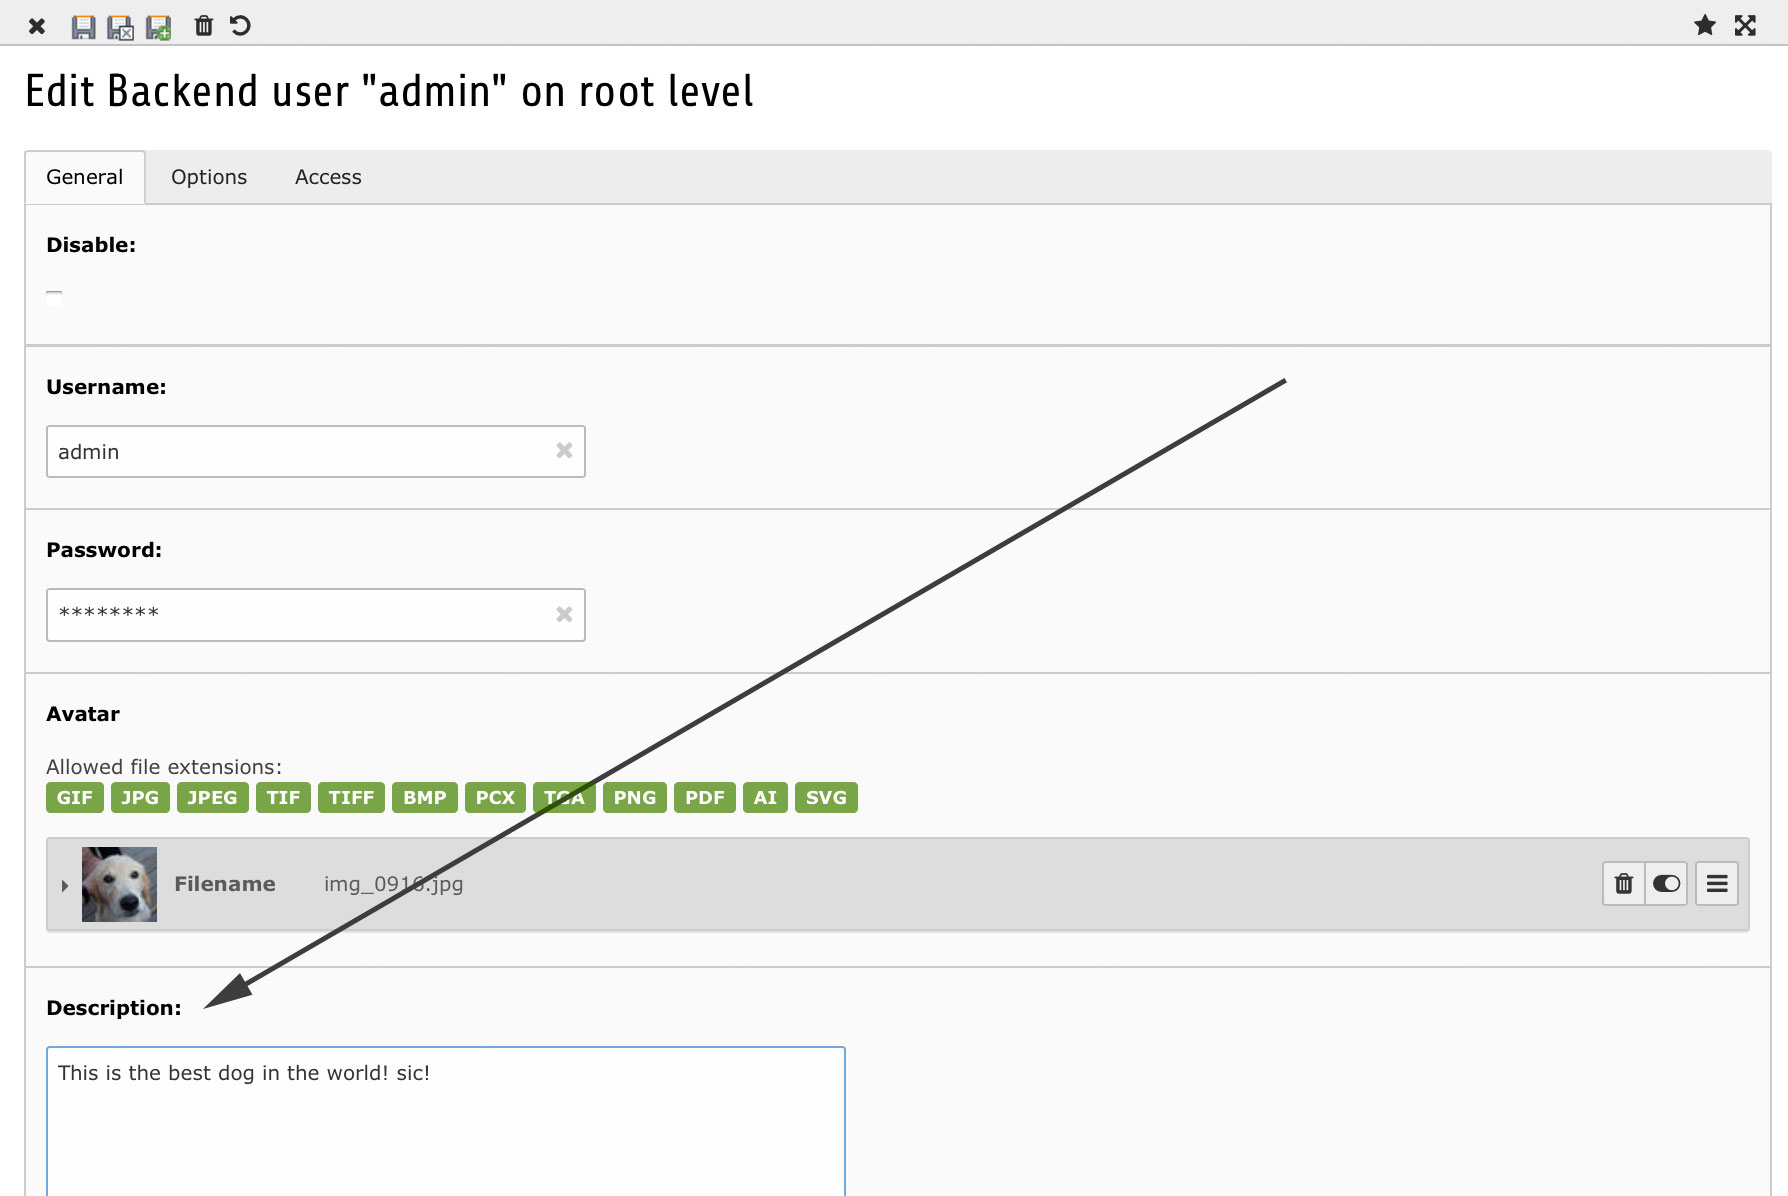
\includegraphics[width=0.6\linewidth]{BackendUserInterface/67578.jpg}
	\end{figure}

\end{frame}

% ------------------------------------------------------------------------------
% LTXE-SLIDE-START
% LTXE-SLIDE-UID:		83db5442-fa2edfcc-925dd5b6-4afe26f5
% LTXE-SLIDE-ORIGIN:	649bd9ee-240381c8-950424ea-f032775b German
% LTXE-SLIDE-TITLE:		Feature: #67603 - Introduce TCA > ctrl > descriptionColumn
% LTXE-SLIDE-REFERENCE:	Feature-67603-IntroduceTcaDescriptionColumn.rst
% ------------------------------------------------------------------------------
\begin{frame}[fragile]
	\frametitle{Interfaz de Usuario de Backend}
	\framesubtitle{Descripción para las Columnas de Tabla}

	Configurando una columna (usualmente \texttt{descripción}) en la configuración de TCA \texttt{['TCA']['ctrl']['descriptionColumn']},
	una descripción puede ser mostrada (mejora la usabilidad para editores y administradores).

	\begin{figure}
		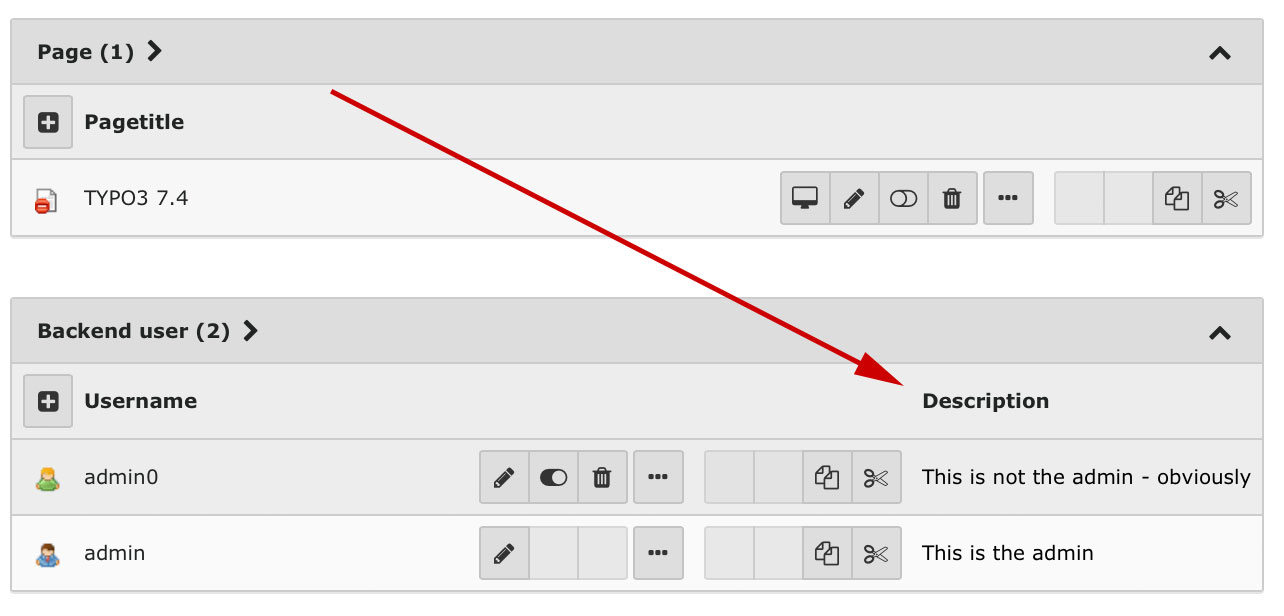
\includegraphics[width=0.7\linewidth]{BackendUserInterface/67603.jpg}
	\end{figure}

\end{frame}

% ------------------------------------------------------------------------------
% LTXE-SLIDE-START
% LTXE-SLIDE-UID:		7c5400a9-c4b667f3-1a0c046a-9dd3b6a9
% LTXE-SLIDE-ORIGIN:	2eeaec46-1929743b-8e6f9285-13d20d3c German
% LTXE-SLIDE-TITLE:		Feature: #59570 - Add description-field for filemounts
% LTXE-SLIDE-REFERENCE:	Feature-59570-AddDescriptionFieldForFilemounts.rst
% ------------------------------------------------------------------------------
\begin{frame}[fragile]
	\frametitle{Interfaz de Usuario de Backend}
	\framesubtitle{Descripción para Puntos de Montajes de ficheros}

	Un nuevo campo "Descripción" se ha añadido a los registros de puntos de montaje de ficheros.
	El campo permite a administradores añadir una descripción corta de la utilidad de un cierto punto de montaje de ficheros,
	qué documentos puede contener, etc.

	\begin{figure}
		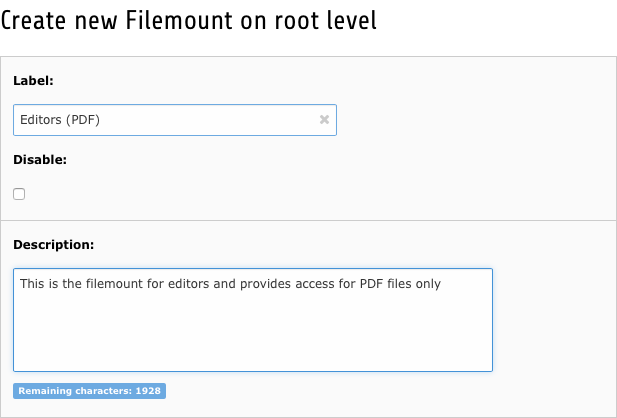
\includegraphics[width=0.55\linewidth]{BackendUserInterface/59570.png}
	\end{figure}

\end{frame}

% ------------------------------------------------------------------------------
% LTXE-SLIDE-START
% LTXE-SLIDE-UID:		d00f63c4-05272792-21a0a301-4d6a726c
% LTXE-SLIDE-ORIGIN:	879b1dda-9167d830-373f7457-0391ebee German
% LTXE-SLIDE-TITLE:		Feature: #68197 - Show a dialog for existing files on upload
% LTXE-SLIDE-REFERENCE:	Feature-68197-ShowADialogForExistingFilesOnUpload.rst
% ------------------------------------------------------------------------------
\begin{frame}[fragile]
	\frametitle{Interfaz de Usuario de Backend}
	\framesubtitle{Diálogo para Ficheros Existentes en Subida}

	Si la subida de un fichero sobreescribiera un fichero existente, se muestra un diálogo, preguntando al usuario
	elegir una acción (p.e. reemplazar, renombrar u omitir).

	\begin{figure}
		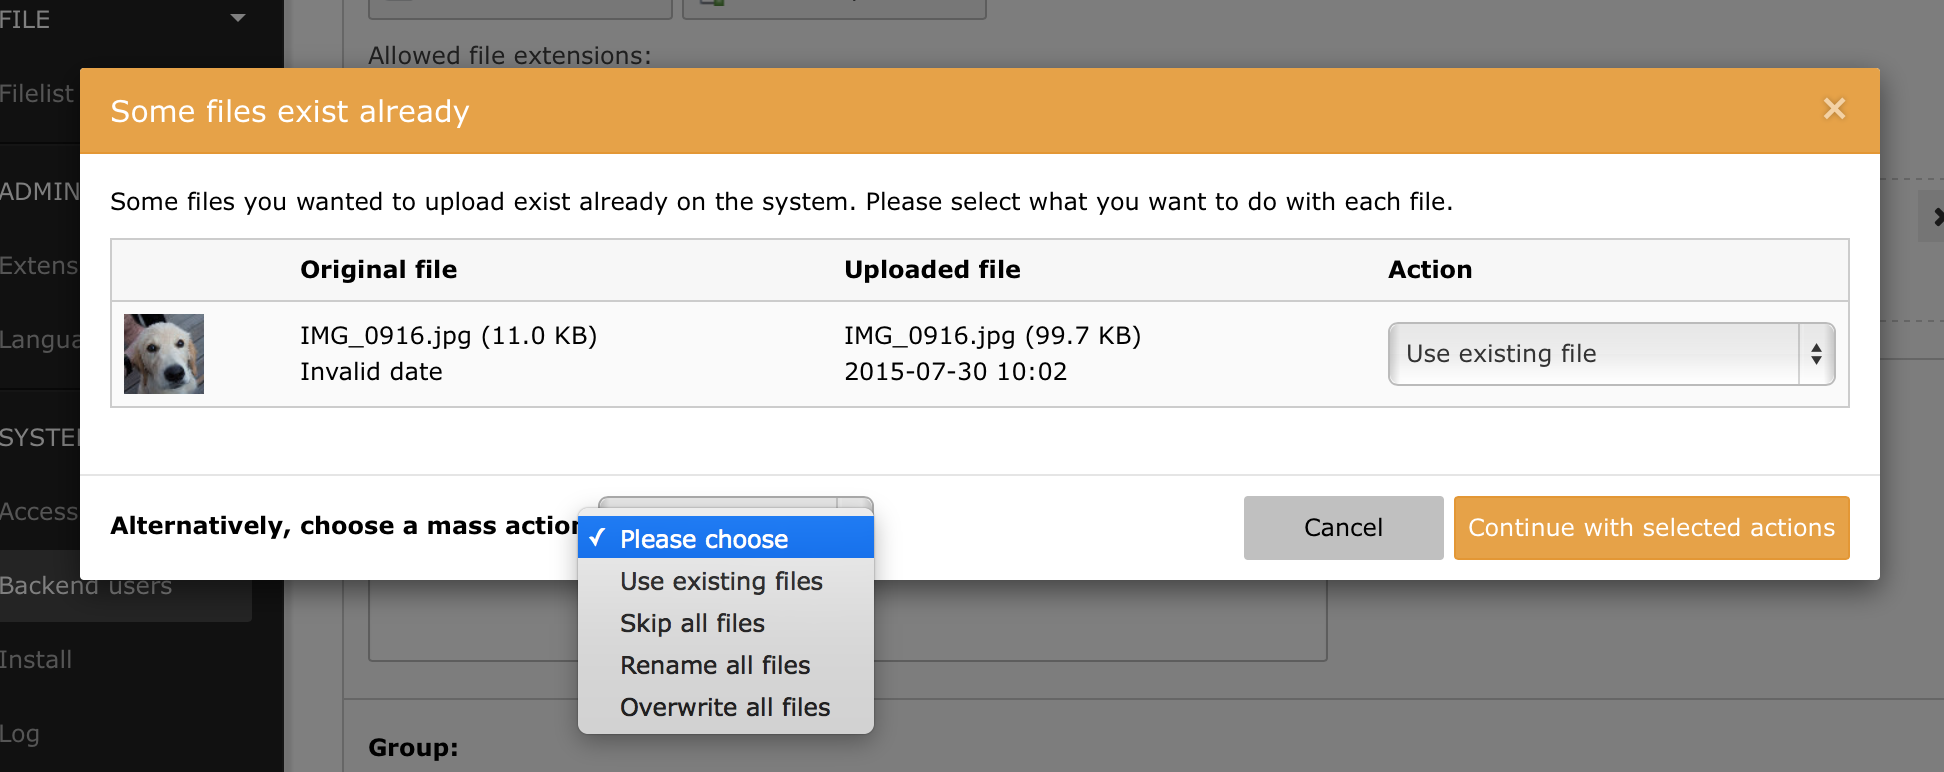
\includegraphics[width=0.9\linewidth]{BackendUserInterface/68197.png}
	\end{figure}

\end{frame}


% ------------------------------------------------------------------------------
% LTXE-SLIDE-START
% LTXE-SLIDE-UID:		31d7dd8e-a3c71be4-309850ab-45a7db72
% LTXE-SLIDE-ORIGIN:	f4baa7b8-2237ad1d-5c4be365-a845f207 German
% LTXE-SLIDE-TITLE:		Feature: #68218 - Lock edit for tt_content
% LTXE-SLIDE-REFERENCE:	Feature-68218-LockEditForTt_content.rst
% ------------------------------------------------------------------------------
\begin{frame}[fragile]
	\frametitle{Interfaz de Usuario de Backend}
	\framesubtitle{Restricción de Edición de Elementos de Contenido (1)}

	Ahora pueden restringirse elementos de contenido para ser editables sólo por administradores
	(similar a la función "Restringir edición a non-Admins" para páginas).
\end{frame}

% ------------------------------------------------------------------------------
% LTXE-SLIDE-START
% LTXE-SLIDE-UID:		31d7dd8e-a3c71be4-309850ab-45a7db72
% LTXE-SLIDE-ORIGIN:	f4baa7b8-2237ad1d-5c4be365-a845f207 German
% LTXE-SLIDE-TITLE:		Feature: #68218 - Lock edit for tt_content
% LTXE-SLIDE-REFERENCE:	Feature-68218-LockEditForTt_content.rst
% ------------------------------------------------------------------------------
\begin{frame}[fragile]
	\frametitle{Interfaz de Usuario de Backend}
	\framesubtitle{Restricción de Edición de Elementos de Contenido (2)}

	\begin{figure}
		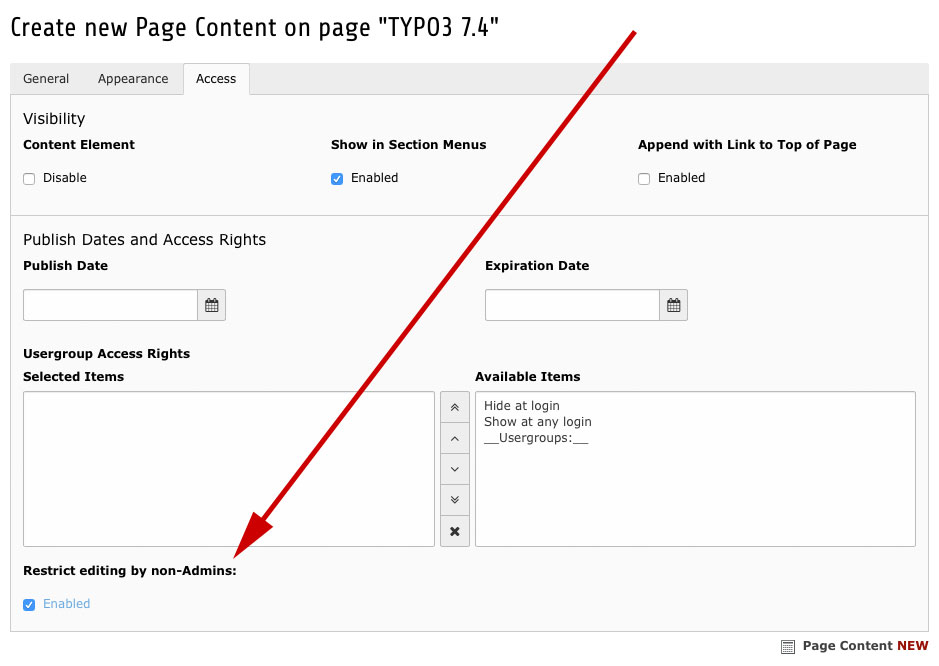
\includegraphics[width=0.6\linewidth]{BackendUserInterface/68218.jpg}
	\end{figure}

\end{frame}

% ------------------------------------------------------------------------------
% LTXE-SLIDE-START
% LTXE-SLIDE-UID:		4e60055a-266e3e24-7baa1613-1226575e
% LTXE-SLIDE-ORIGIN:	bc83e40f-9b7bac03-ea5f07c4-be27eb56 German
% LTXE-SLIDE-TITLE:		Feature: #68315 - Include pageTSconfig file (1)
% LTXE-SLIDE-REFERENCE:	Feature-68315-IncludeAPageTSconfigFileInPagePropertiesLikeTSStaticTemplates.rst
% ------------------------------------------------------------------------------
\begin{frame}[fragile]
	\frametitle{Interfaz de Usuario de Backend}
	\framesubtitle{Incluir Ficheros Estáticos TSconfig (1)}

	En las propiedades de página una opción permite incluir un fichero TSconfig de página
	(del mismo modo que se incluyen plantillas estáticas TypoScript).

	\begin{figure}
		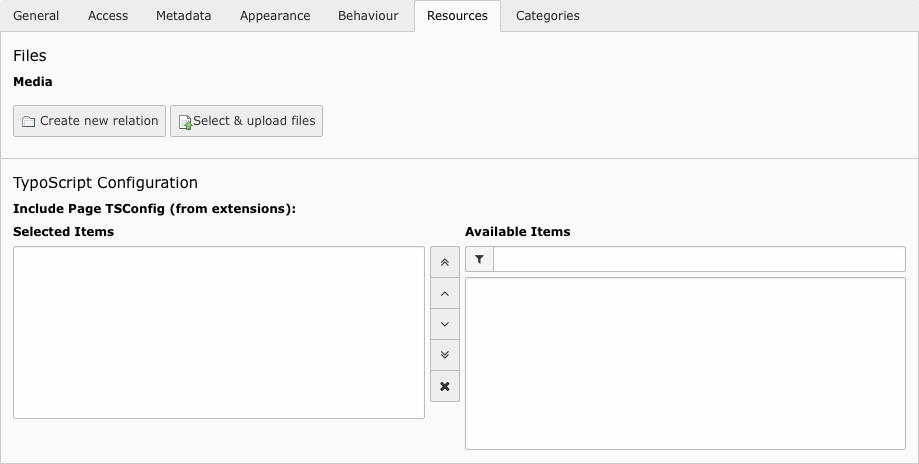
\includegraphics[width=0.8\linewidth]{BackendUserInterface/68315.png}
	\end{figure}

\end{frame}

% ------------------------------------------------------------------------------
% LTXE-SLIDE-START
% LTXE-SLIDE-UID:		4f5cb411-3ea84dfd-84edb16d-433b9fc5
% LTXE-SLIDE-ORIGIN:	9b7bac03-ea5f07c4-be27eb56-ac03e27e German
% LTXE-SLIDE-TITLE:		Feature: #68315 - Include pageTSconfig file (2)
% LTXE-SLIDE-REFERENCE:	Feature-68315-IncludeAPageTSconfigFileInPagePropertiesLikeTSStaticTemplates.rst
% ------------------------------------------------------------------------------
\begin{frame}[fragile]
	\frametitle{Interfaz de Usuario de Backend}
	\framesubtitle{Incluir Ficheros Estáticos TSconfig (2)}

	% decrease font size for code listing
	\lstset{basicstyle=\tiny\ttfamily}

	El siguiente método registra un fichero TSconfig de página:

	\begin{lstlisting}
		\TYPO3\CMS\Core\Utility\ExtensionManagementUtility::registerPageTSConfigFile(
		  'extension_name',
		  'Configuration/PageTS/myPageTSconfigFile.txt',
		  'My special configuration'
		);
	\end{lstlisting}

\end{frame}

% ------------------------------------------------------------------------------
% LTXE-SLIDE-START
% LTXE-SLIDE-UID:		c00b2bfd-2c1b02b0-a7ef9cd0-62f147d2
% LTXE-SLIDE-ORIGIN:	f8d888b1-b93dcf4a-e20b976e-9a5c277e German
% LTXE-SLIDE-TITLE:		Feature: #68395 - Allow real copies of content elements into foreign languages
% LTXE-SLIDE-REFERENCE:	Feature-68395-AllowRealCopiesOfContentElementsIntoForeignLanguages.rst
% ------------------------------------------------------------------------------
\begin{frame}[fragile]
	\frametitle{Interfaz de Usuario de Backend}
	\framesubtitle{Copias Reales de Elementos de Contenido}

	Se ha añadido un nuevo botón a cada columna en el módulo "Página" que permite copias \textit{reales} de elementos de contenido
	en un lenguaje (no sólo referencias).

	\begin{figure}
		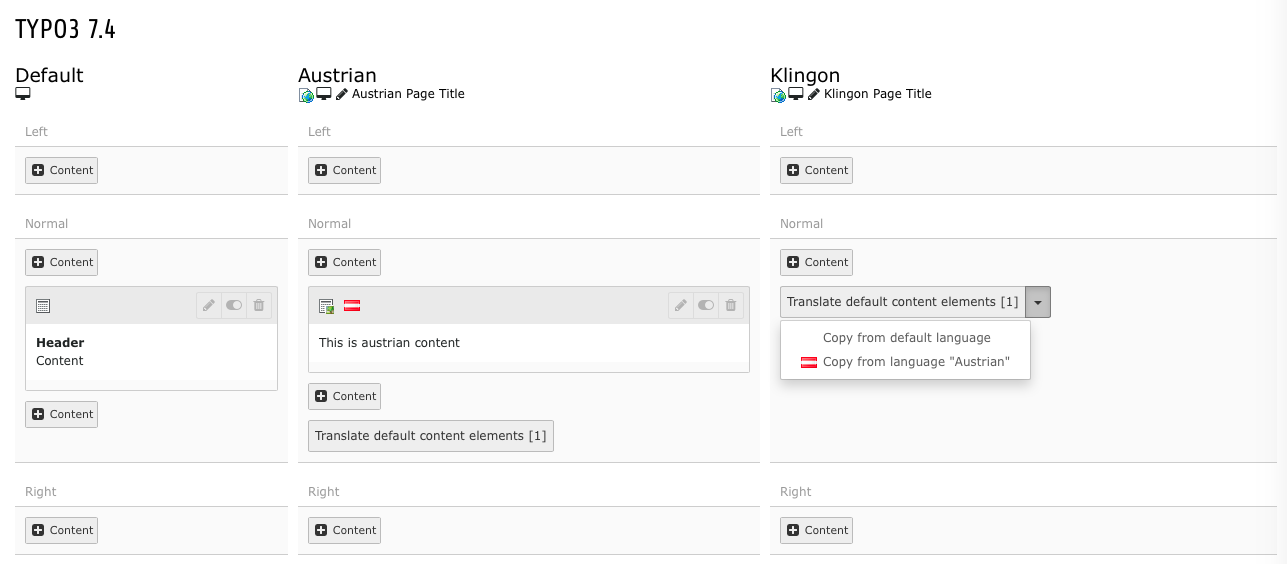
\includegraphics[width=0.9\linewidth]{BackendUserInterface/68395.png}
	\end{figure}

\end{frame}


